\section{Results}
\noindent
We generated the visibility graph parameters for three tectonic seismic regions in northern Iran for the period 2005-15. The number of earthquakes in each catalog after declustering and their seismicity parameters is presented in Table.~\ref{tab:b_k_m_param}. 

\begin{table}[h]
\centering
\caption{Declustered number of earthquakes, seismic parameters and $k-M$ slope values for north Iran tectonic seismic zones.}
\begin{tabular}{ccccc}
Region          & Number of Earthquake &  $Mc$ &  $b-value$ & $k-M$ slope \\ \hline
Azerbaijan     & 93                                 & 3.5   & 1.0190  & 9.2004       \\ \hline
Alborz            & 794                               & 2.6   & 0.7717  & 9.0461      \\ \hline
Kopeh Dagh  & 282                               & 2.6   & 0.5799  & 6.5818     \\ \hline
\end{tabular}
\label{tab:b_k_m_param}
\end{table}

\noindent
Fig.~\ref{fig:k_m_plot_m}  shows the  $k-M$  relationship for the study regions. We categorized magnitudes in small magnitude bins ($\Delta M=0.1$). It is clear from the Fig.~\ref{fig:mag-time} that the specific magnitude bin can result in different connectivity degrees regarding the occurring time of the earthquake event. In general, with increasing magnitude, the connectivity degree increases, which increases the slope of the  $k-M$  relationship. 

\begin{figure} [ht]
\centering
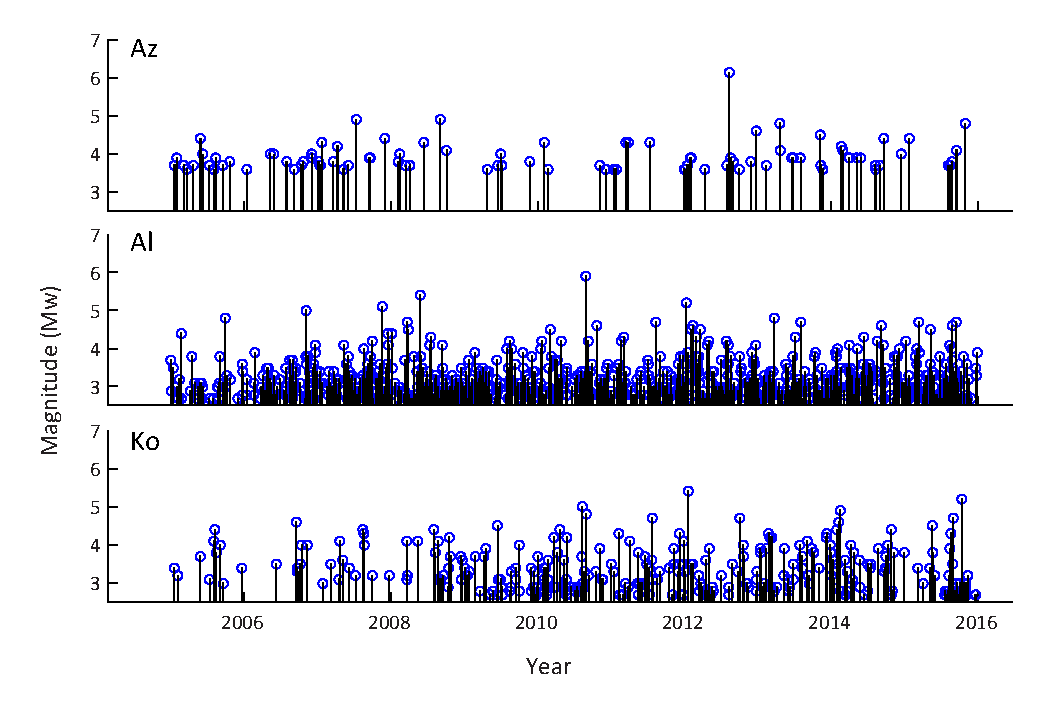
\includegraphics[scale=0.35]{figures/pdf/Figure06.pdf} 
\caption{ $k-M$ relationship for north Iran tectonic seismic regions. The blue circles indicate the connectivity degrees. The red line is the linear regression line fits the data. The numbers on the lines is the slope of the lines.}
\label{fig:k_m_plot_m}
\end{figure}
 \noindent
We compared the  $k-M$  slope with the  $b-value$  of the Gutenberg-Richter law through the entire catalog and in the sliding windows in time. The  $b-value$  is generated through the maximum likelihood estimation  \citep{Aki1965} .

\begin{equation}
b = \frac{log_{10}(e) }{\overline{M} - M_{min}},
\end{equation}
 \noindent
where $\overline{M}$ is the average magnitude, and  $M_ {min}$ is the minimum magnitude in the sample, which in this case is the completeness magnitude for each tectonic seismic region. The number of sequences and threshold magnitudes is considerably different for all tectonic seismic regions.  \citet{Telesca2013}  studied the effect of the number of earthquakes in the catalog on the  $k-M$  slope. Comparing the result with the Guerrero region with reduced random sequence,  \citet{Telesca2013}  found that the number of sequences did not affect the  $k-M$  slope.  According to  \citet{Telesca2012}, the threshold magnitude has minor effect in the VG parameters. In order to analyze the sensitivity of the catalogs to the number of events and the threshold magnitude, we randomly picked 200 sequences from the catalogs with various sequence sizes. The minimum size of random windows is 150 events. (Note that the number of events in each catalog, before removing the events with magnitude less than the completeness magnitude, is 271, 1262, and 399 for Azerbaijan, Alborz, and Kopeh Dagh regions, respectively.). The maximum size is the size of the entire catalog. For each randomly picked magnitude time series,  we estimate $Mc$; then the $k-M$  and $b-value$ are calculated. Fig.~\ref{fig:random} shows the relationship between  $k-M$  slope and  $b-value$  of the randomly selected data and the statistical parameters for variables. Although changing the number of events and the threshold magnitude is slightly changing the results, however,  the results are fairly well clustered for each tectonic seismic region. 
   
 \begin{figure} [ht]
\centering
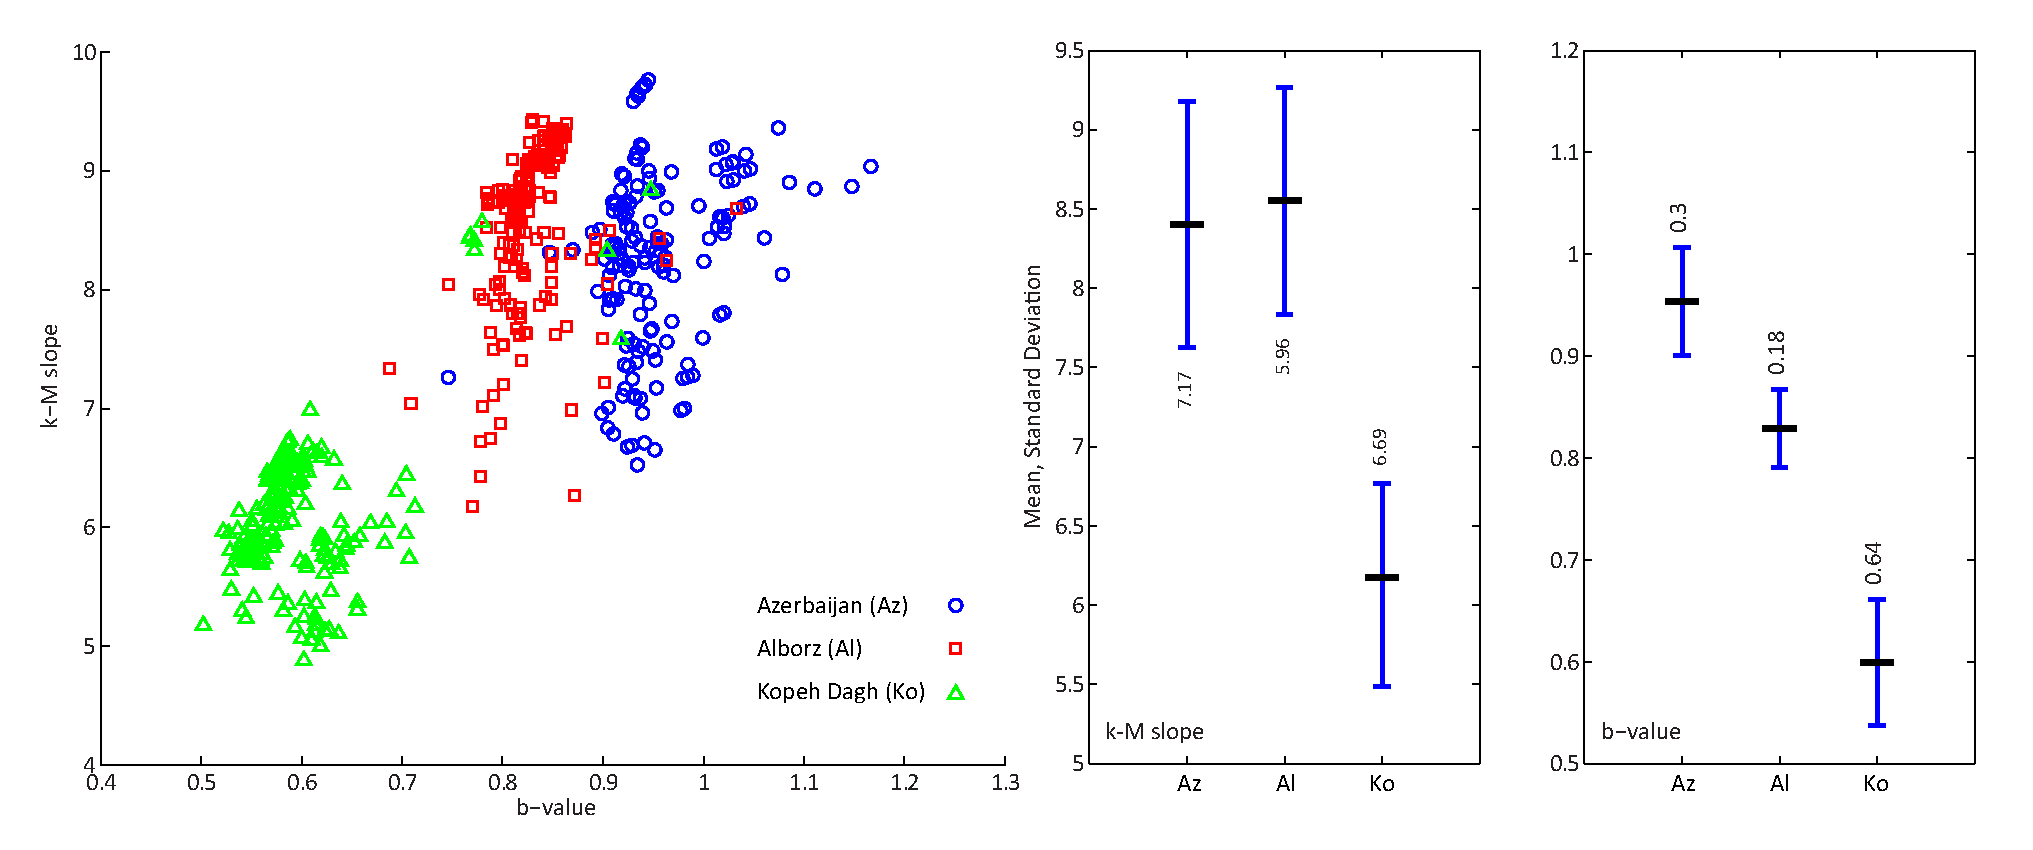
\includegraphics[scale=0.5]{figures/pdf/Figure07.pdf} 
\caption{ Relationship between $k-M$ and $b-value$ of three Iranian tectonic seismic regions for 200 random sequence. The numbers on the mean and standard deviation plots are coefficient of variations in percent $(standard \ deviation / mean)$.}
\label{fig:random}
\end{figure}

\noindent
The coefficient of variation of parameters is shown in Fig.~\ref{fig:random}. The  $k-M$  slope shows the higher coefficient of variation which indicates the fact that the  $k-M$  slope is more dependent on the window size and threshold magnitude than on the a-  and  b-values , which suggests that  the $k-M$  slope can better represent the dynamic characteristics of the magnitude-time series. 
 \noindent
 Fig.~\ref{fig:regression} shows the relationship between the  $k-M$  slope and $b-value$ for the three tectonic seismic regions in northern Iran and three other studies of Mexican zones  \citep{Telesca2013}, Pannonia zones  \citep{Telesca2014}, and synthetic data \citep{Telesca2014-pone}. Adding the results of the current study into the results of three previous similar studies improves the regression factor, and empowers the concept of the universal character of the relationship between the  $b-value$  and the  $k-M$  slope, as  \citet{Telesca2014} concluded. 
 
\begin{figure} [ht]
\centering
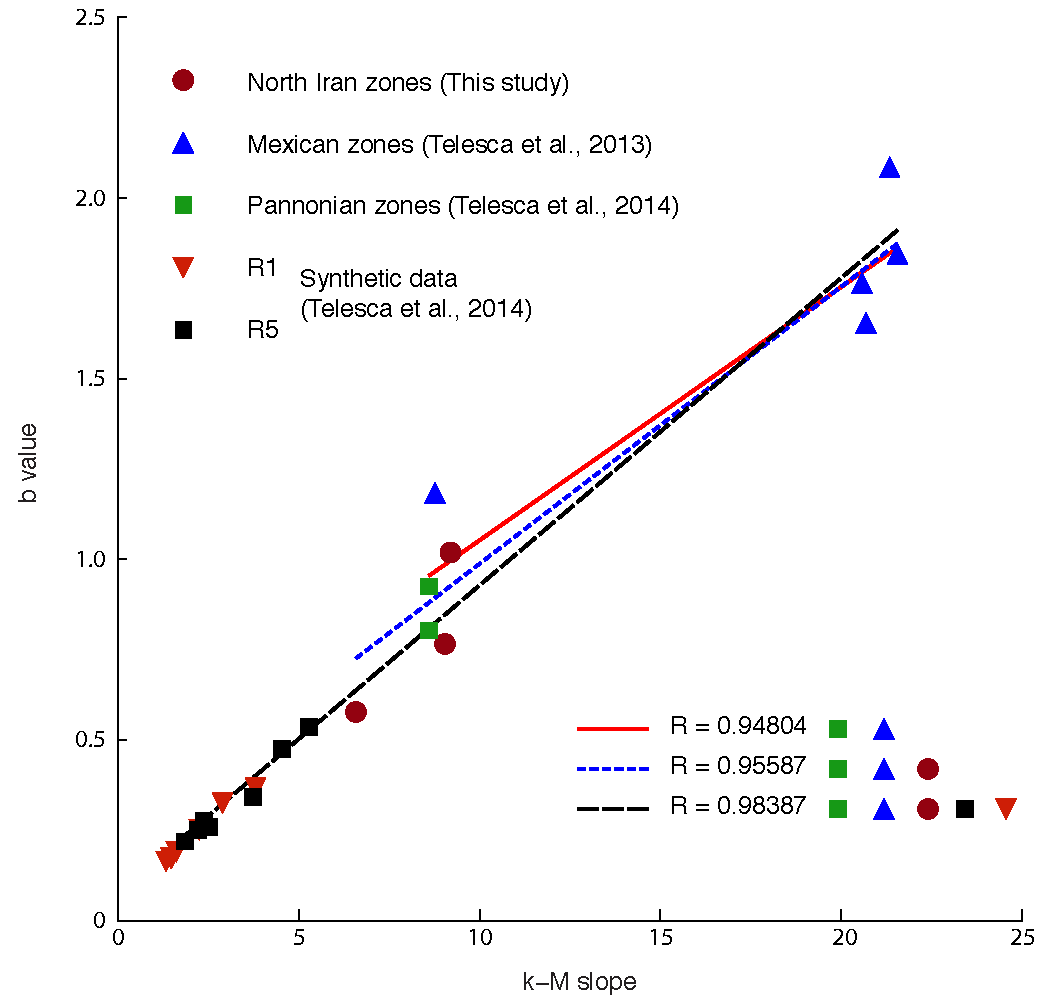
\includegraphics[scale=0.6]{figures/pdf/Figure08.pdf} 
\caption{ Relationship between $k-M$ slope and $b-value$ of three Iranian tectonic seismic zones (this study) and three other studies of Mexican zones \citep{Telesca2013}, Pannonia zones \citep{Telesca2014}, and synthetic data \citep{Telesca2014-pone}. The lines represent the linear regression fit of data. The correlation coefficients (R) are represented for different combination of data.}
\label{fig:regression}
\end{figure}

\noindent
Fig.\ref{fig:tc} shows the variation of the  $k-M$  slope and  $b-value$  with time. Having a lower number of events, we chose 20 events as the window length with a shift of one event between two successive windows. The calculated parameters of each window were associated with the time of occurrence of the last event in the sliding window. The  $k-M$  slope and  $b-value$  in all tectonic seismic regions are very similar. In general, in all regions the $b-value$  and  $k-M$  slope drop considerably before large earthquakes. The decline in the  $b-value$  before large earthquakes has been studied in many regions \citep{Wyss2000, Wyss2006, Schorlemmer2005, Chan2012}.
\noindent
\citet{Telesca2016}  observed the decrease in  $<T_C>$  before the large earthquake of the western India earthquake sequence. Fig.\ref{fig:tc}  shows the time variation of  $<T_C>$   in the study area. The reduction of  $<T_C>$   before large earthquakes is clearly visible.  \citet{Telesca2016}  demonstrated that the decrement of  $<T_C>$   before a large earthquake is independent of window size and threshold magnitude. Decreasing the value of  $<T_C>$  ,  $k-M$ , and  $b-value$  before large earthquakes predominantly happened in all tectonic seismic regions (see Fig.\ref{fig:tc} for reference.)
 
  
 \begin{figure} [ht]
\centering
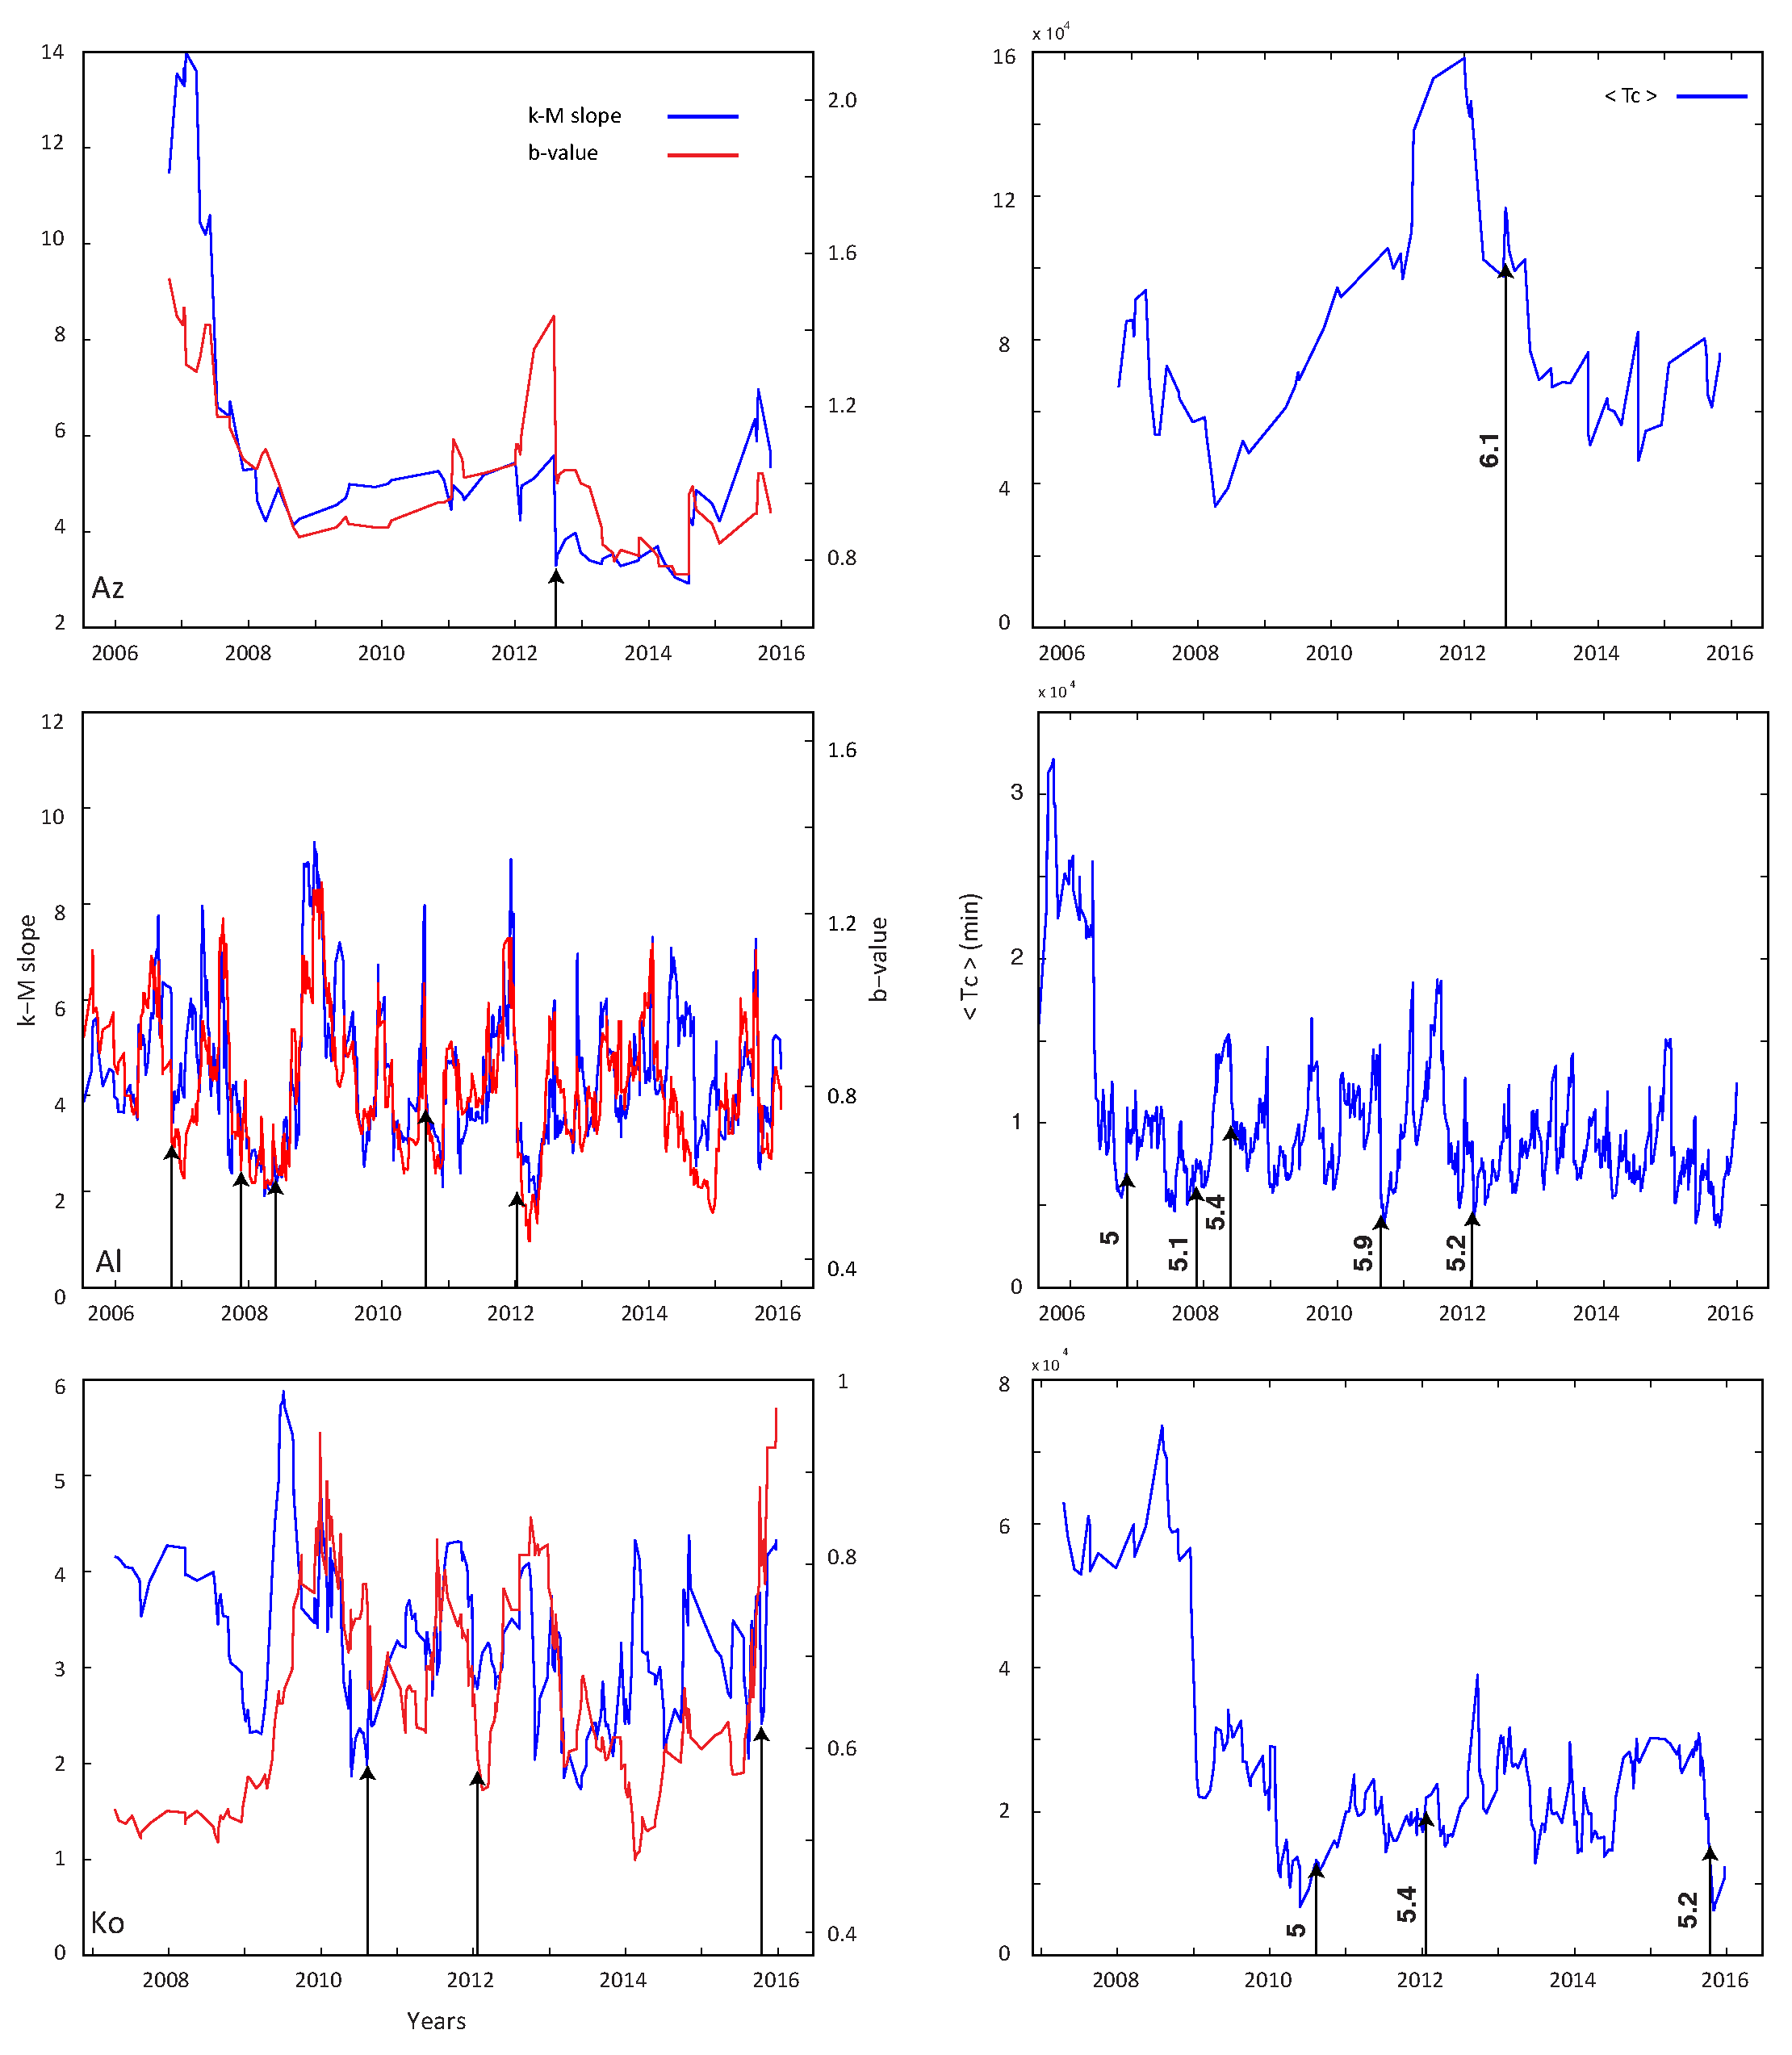
\includegraphics[scale=0.4]{figures/pdf/Figure09.pdf} 
\caption{ Variation of $k-M$ slope  and $b-value$ (Left), and $ < T_C >$ (Right) as a function of time for three tectonic seismic regions in north Iran. Black arrows show the occurrence of the major earthquakes. Numbers on arrows indicate the moment magnitude of the earthquake (see Fig.~\ref{fig:mag-time} for reference). Decreasing the value of  $<T_C>$  ,  $k-M$ , and  $b-value$  before large earthquakes predominantly happened in all tectonic seismic regions.}
\label{fig:tc}
\end{figure}
 
 % Original text
%\section{Results}
%\noindent
%We generated the visibility graph parameters for three tectonic seismic regions in northern Iran for the period from 2005 to 2015. Number of earthquakes in each catalog after declustering and the seismicity parameters are presented in Table.~\ref{tab:b_k_m_param}. 
%
%
%\begin{table}[h]
%\centering
%\caption{Seismic parameters and $k-M$ slope values for north Iran tectonic seismic zones.}
%\begin{tabular}{ccccc}
%Region          & Number of Earthquake &  $Mc$ &  $b-value$ & $k-M$ slope \\ \hline
%Azerbaijan     & 93                                 & 3.5   & 1.0190  & 9.2004       \\ \hline
%Alborz            & 794                               & 2.6   & 0.7717  & 9.0461      \\ \hline
%Kopek Dagh  & 282                               & 2.6   & 0.5799  & 6.5818     \\ \hline
%\end{tabular}
%\label{tab:b_k_m_param}
%\end{table}
%
%\noindent
%Fig.~\ref{fig:k_m_plot_m} shows the $k-M$ relationship for the study regions.  In general with increasing magnitude the connectivity degree increases which results in increasing the slope of the $k-M$ relationship. 
%
%\begin{figure} [ht]
%\centering
%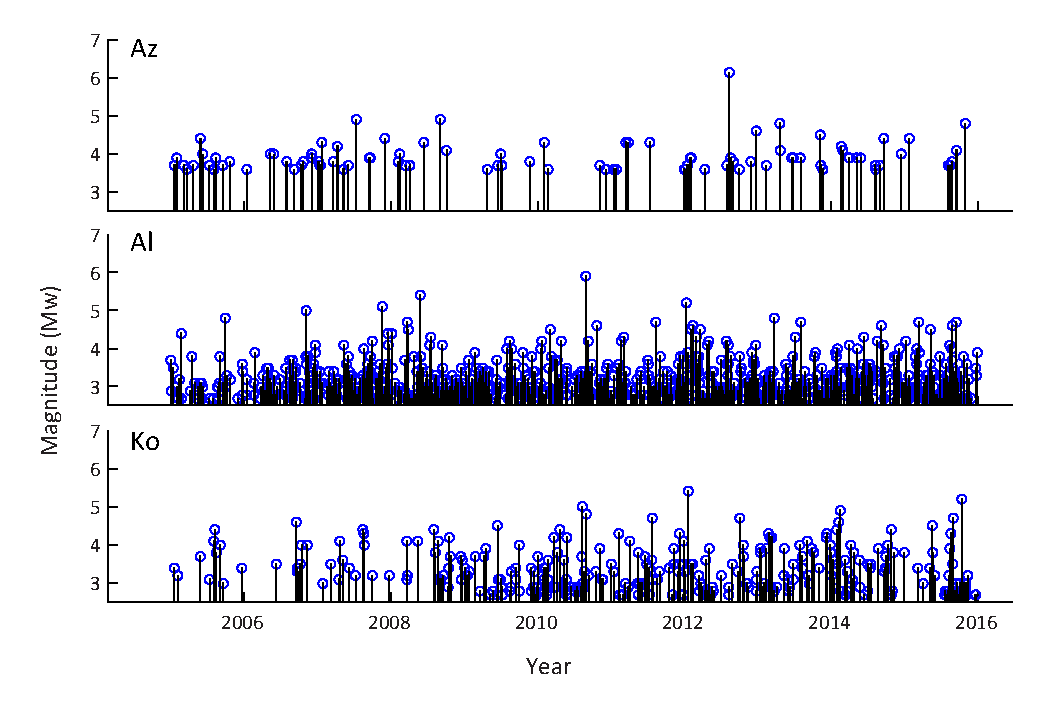
\includegraphics[scale=0.35]{figures/pdf/Figure05.pdf} 
%\caption{ $k-M$ relationship for north Iran seismicity. a) Azerbaijan b) Alborz c)Kopeh Dagh}
%\label{fig:k_m_plot_m}
%\end{figure}
%
%\noindent
%We compared the $k-M$ slope with the $b-value$ of the Gutenberg-Richter law in the whole catalog and also in the sliding windows in time. The $b-value$ is generated through the maximum likelihood estimation \citep{Aki1965}.
%
%\begin{equation}
%b = \frac{log_{10}(e) }{\overline{M} - M_{min}},
%\end{equation}
% 
% \noindent
% where $\overline{M}$ is the average magnitude and $M_{min}$ is the minimum magnitude in the sample, which in this case is the completeness magnitude for each tectonic seismic zone. Number of sequences and threshold magnitudes are considerably different for all tectonic seismic regions. \citet{Telesca2013} studied the effect of the number of earthquakes in catalog on the $k-M$ slope. Comparing the result of Guerrero region with reduced random sequence, \citet{Telesca2013} found that the number of sequence doesn't affect the $k-M$ slope.  According to \citet{Telesca2012}, the threshold magnitude has a minor effect in the VG parameters. In order to analyze the sensitivity of the catalogs to the number of events and the threshold magnitude we randomly pick 200 sequences from the catalogs with various sequence size. The minimum size of random windows are 150 events (note that the number of events in each catalog, before removing the events with magnitude less than completeness magnitude, are 271, 1262, and 399 for Azerbaijan, Alborz, and Kopeh Dagh regions, respectively) and the maximum size is the size of the whole catalog. For each randomly picked magnitude time series we estimate the $Mc$ and calculated the $k-M$ and $b-value$. Fig.~\ref{fig:random} shows the relationship between $k-M$ slope and $b-value$ of the randomly selected data and statistical parameters for variables. Although changing the number of events and the threshold magnitude are slightly changes the results, they are fairly well clustered for each tectonic seismic region. 
% 
% \begin{figure} [ht]
%\centering
%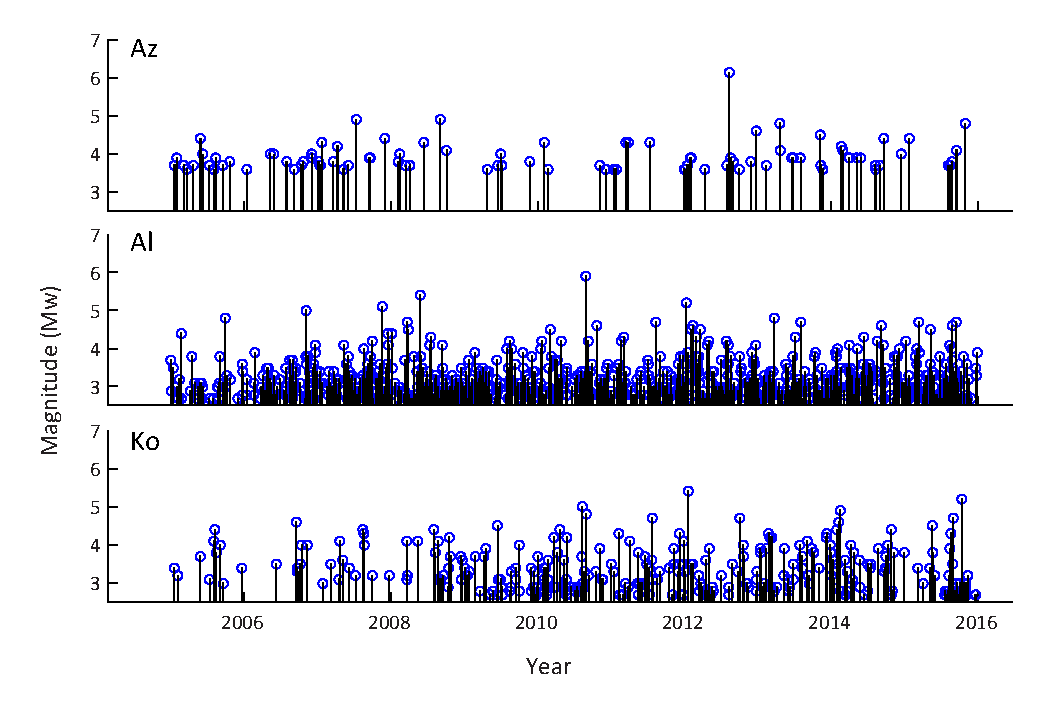
\includegraphics[scale=0.4]{figures/pdf/Figure06.pdf} 
%\caption{ Relationship between $k-M$ and $b-value$ of three Iranian tectonic seismic regions for 200 random sequence. The numbers on the mean and standard deviation plots are coefficient of variations in percent$(standard \ deviation / mean)$.}
%\label{fig:random}
%\end{figure}
% 
% \noindent
%The coefficient of variation of parameters are shown in Fig.~\ref{fig:random}. The $k-M$ slope shows higher coefficient of variation. We may argue that the $k-M$ slope is much dependent to the window size and threshold magnitude than $a-$ and $b-value$, which suggest the idea that $k-M$ slope can better represent the dynamic characteristics of the magnitude-time series. 
% 
% 
%
% 
% \noindent
% Fig.~\ref{fig:regression} shows the relationship between the $k-M$ slope for three tectonic seismic regions in north of Iran and two other studies of Mexican zones \citep{Telesca2013}, and Pannonia zones \citep{Telesca2014}. Adding the results of the current study into the results of two previous similar studies improves the regression factor (with an increase from R=0.95 to R=0.958) and empower the idea of universal character of the relationship between the $b-value$ and the $k-M$ slope as \citet{Telesca2014} concluded. 
%
%\begin{figure} [ht]
%\centering
%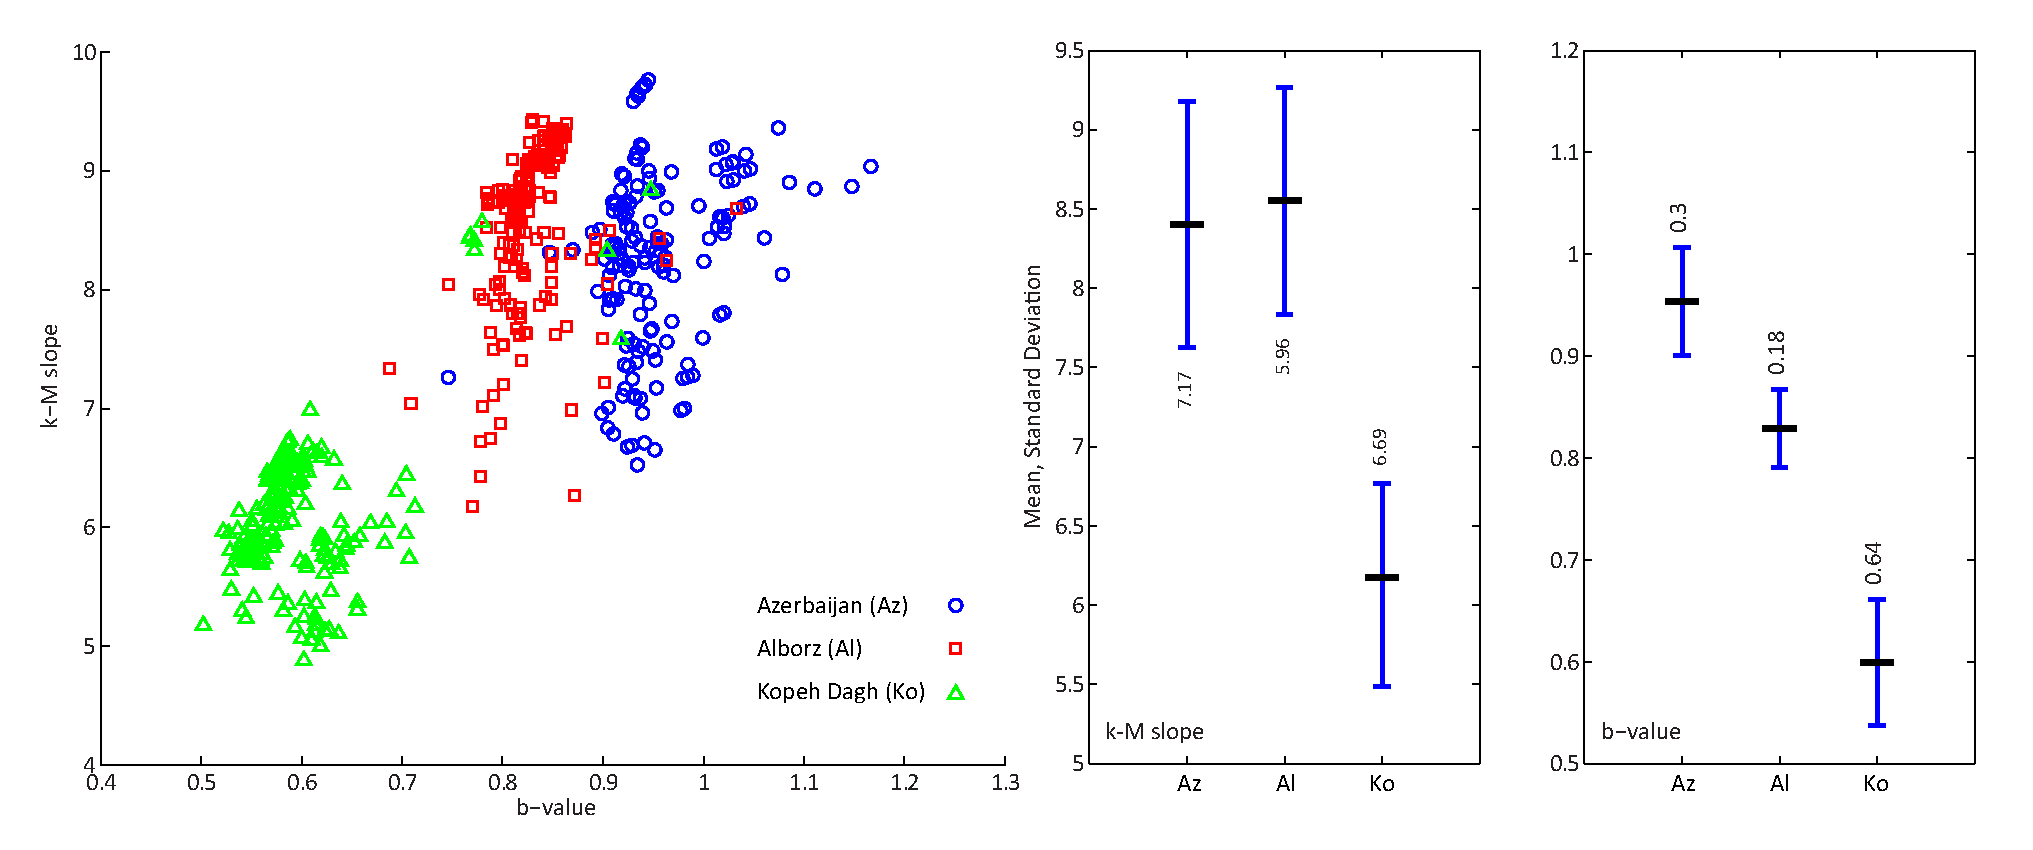
\includegraphics[scale=0.3]{figures/pdf/Figure07.pdf} 
%\caption{ Relationship between $k-M$ and $b-value$ of three Iranian tectonic seismic zones (this study) and two other studies of Mexican zones \citep{Telesca2013}, and Pannonia zones \citep{Telesca2014}. The dashed red line shows the regression line for data of  Mexican zones and Pannonia zones \citep{Telesca2014}, and the solid blue line shows the regression line for data of all regions (Mexican, Pannonian and north Iran)}
%\label{fig:regression}
%\end{figure}
%
%
%\noindent 
%Fig.\ref{fig:tc}  shows the variation of the $k-M$ slope and $b-value$ with time. Having lower number of event, we used 20 events as a window length with shift of one event between two successive windows. The calculated parameters of each window was associated with the time of occurrence of the last event in sliding window. There is a very good similarity between the $k-M$ slope and $b-value$ in all tectonic seismic regions. In general, In all regions the $b-value$ and $k-M$ slope considerably drop before big earthquakes. Dropping the $b-value$ before large earthquakes have been studied in many different region \citep[e.g.][]{Wyss2000,Wyss2006,Schorlemmer2005,Chan2012}
%
%\noindent
%\citet{Telesca2016} observed the decreasing in $<Tc>$ before large earthquake of Western India earthquake sequence. Fig.~\ref{fig:tc} shows the time variation of $<Tc>$ in the study area and decrease in $<Tc>$ befor large earthquakes is clearly visible. \citet{Telesca2016} demonstrated that the decrement of $<Tc>$ before large earthquake are independent of window size and the threshold magnitude. Fig.~\ref{fig:tc} shows the decrement of value of $< T_C >$, $k-M$, and $b-value$ before big earthquakes.
% 
% \begin{figure} [ht]
%\centering
%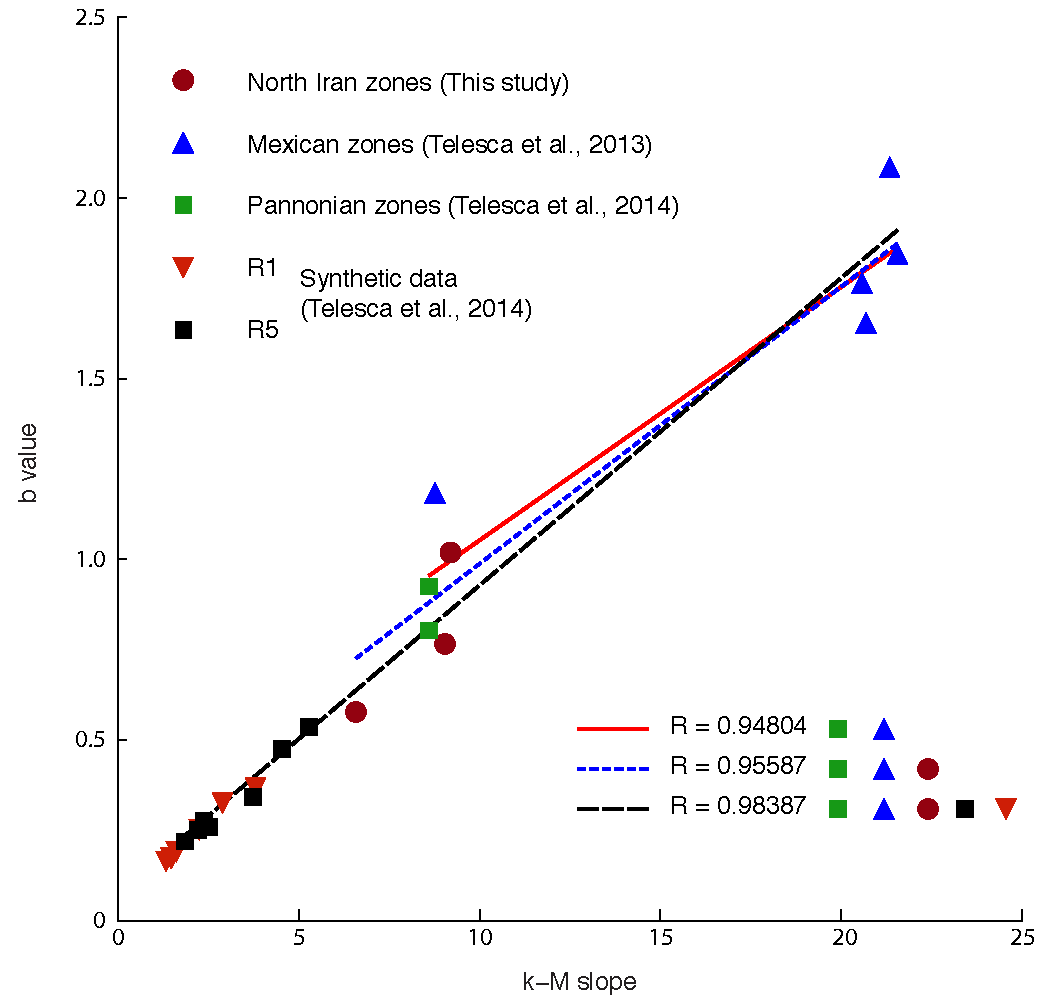
\includegraphics[scale=0.34]{figures/pdf/Figure08.pdf} 
%\caption{ Variation of $k-M$ slope  and $b-value$ (Left), and $ < T_C >$ (Right) with time. Black arrows show the occurrence of the major earthquakes. Numbers on arrows indicate the moment magnitude of the earthquake.}
%\label{fig:tc}
%\end{figure}
 
 
 
 
 
 
 